\chapter{Pion photoproduction}\label{sec:PionPhotoproduction}
We now consider the case of pion photoproduction. In the model mentioned in section \ref{sec:model} the nucleon is in a superposition of states with an arbitrary number of pions but we constrain the model to the one-pion approximation. This is illustrated on figure \ref{Multicomponent}
\begin{marginfigure}
	\centering
	

% Pattern Info

\tikzset{
	pattern size/.store in=\mcSize, 
	pattern size = 5pt,
	pattern thickness/.store in=\mcThickness, 
	pattern thickness = 0.3pt,
	pattern radius/.store in=\mcRadius, 
	pattern radius = 1pt}
\makeatletter
\pgfutil@ifundefined{pgf@pattern@name@_t53nej2q6}{
	\makeatletter
	\pgfdeclarepatternformonly[\mcRadius,\mcThickness,\mcSize]{_t53nej2q6}
	{\pgfpoint{-0.5*\mcSize}{-0.5*\mcSize}}
	{\pgfpoint{0.5*\mcSize}{0.5*\mcSize}}
	{\pgfpoint{\mcSize}{\mcSize}}
	{
		\pgfsetcolor{\tikz@pattern@color}
		\pgfsetlinewidth{\mcThickness}
		\pgfpathcircle\pgfpointorigin{\mcRadius}
		\pgfusepath{stroke}
}}
\makeatother
\tikzset{every picture/.style={line width=0.75pt}} %set default line width to 0.75pt        

\begin{tikzpicture}[x=0.75pt,y=0.75pt,yscale=-1,xscale=1]
	%uncomment if require: \path (0,389); %set diagram left start at 0, and has height of 389
	
	%Flowchart: Connector [id:dp12351893787926194] 
	\draw  [color={rgb, 255:red, 208; green, 2; blue, 27 }  ,draw opacity=1 ][pattern=_t53nej2q6,pattern size=2.925pt,pattern thickness=0.75pt,pattern radius=0.75pt, pattern color={rgb, 255:red, 208; green, 2; blue, 27}][line width=0.75]  (315.75,205) .. controls (315.75,154.6) and (356.6,113.75) .. (407,113.75) .. controls (457.4,113.75) and (498.25,154.6) .. (498.25,205) .. controls (498.25,255.4) and (457.4,296.25) .. (407,296.25) .. controls (356.6,296.25) and (315.75,255.4) .. (315.75,205) -- cycle ;
	%Flowchart: Connector [id:dp2648272257538774] 
	\draw  [color={rgb, 255:red, 0; green, 0; blue, 0 }  ,draw opacity=1 ][fill={rgb, 255:red, 126; green, 211; blue, 33 }  ,fill opacity=1 ][line width=0.75]  (379,205) .. controls (379,189.54) and (391.54,177) .. (407,177) .. controls (422.46,177) and (435,189.54) .. (435,205) .. controls (435,220.46) and (422.46,233) .. (407,233) .. controls (391.54,233) and (379,220.46) .. (379,205) -- cycle ;
	%Shape: Circle [id:dp5293194247132722] 
	\draw  [fill={rgb, 255:red, 255; green, 255; blue, 255 }  ,fill opacity=1 ] (397,151) .. controls (397,145.48) and (401.48,141) .. (407,141) .. controls (412.52,141) and (417,145.48) .. (417,151) .. controls (417,156.52) and (412.52,161) .. (407,161) .. controls (401.48,161) and (397,156.52) .. (397,151) -- cycle ;
	
	% Text Node
	\draw (400,200) node [anchor=north west][inner sep=0.75pt]  [color={rgb, 255:red, 0; green, 0; blue, 0 }  ,opacity=1 ]  {$N$};
	% Text Node
	\draw (401,147) node [anchor=north west][inner sep=0.75pt]  [color={rgb, 255:red, 0; green, 0; blue, 0 }  ,opacity=1 ]  {$\pi $};
	
	
\end{tikzpicture}
	\caption{Illustration of the dressed nucleon. In the centre (green) is a nucleon and surrounding it is a cloud of virtual pions (red gradient). }
	\label{Multicomponent}
\end{marginfigure}
There are four pion photoproduction processes on nucleons and these are given by
\begin{align}
	p \gamma & \rightarrow p \pi^0 \label{photonew1}\\
	p \gamma & \rightarrow n \pi^+ \label{photonew2}\\
	n \gamma & \rightarrow n \pi^0 \label{photonew3}\\
	n \gamma & \rightarrow p \pi^- \label{photonew4}.
\end{align}
Within the framework of this model, we would expect these processes by applying the equation \eqref{isocoeff} to the isospin state of the given nucleon, i.e
\begin{equation} \label{isovectorex}
	(\vec{\tau}\cdot\vec{\pi}) p = p\pi^0 + \sqrt{2}n\pi^+,
\end{equation}
and similarly for the isospin state of the neutron. As mentioned in section \ref{sec:DressingofProton} the pion is trapped behind a potential barrier of height $140$ MeV and cannot leave unless an incoming photon of sufficient energy hits the pion-nucleon system and photodisintegrates the virtual pion and creates a physical pion in the process. This means pion photoproduction comes naturally as a photodisintegration process. Consider some initial bound state represented by the following two-component wave function

\begin{equation} \label{phii}
	\ket{\Phi_i} = \mqty[\phi_p \\ \phi_{N\pi}],
\end{equation}
where $\phi$ represents a bound state. The final state consists of the same superposition but in an unbound system represented by $\psi$, i.e.
\begin{equation} \label{psif}
	\ket{\Psi_f} = \mqty[\psi_p \\ \psi_{N\pi}].
\end{equation}
The two-component wave function photodisintegration is similar to the photodisintegration process of the deuteron\footnote{This is covered in appendix \ref{app:deuteron}}. We can apply a similar approach and get an expression for the total cross section as a function of energy and the strength parameter $S$ and the range parameter $b$. The general idea is to fit the parameters to experimental data such that we get a set of parameters within which the model can describe the total cross-section near the threshold. We constrain the model to only apply near the threshold since we expect more pions are needed to adaquatly describe the total cross section at higher energies.
The advantages of this model are twofold--the reduced number of parameters allows us to easily fit the model to experimental data and the generality of the model allows us to apply these parameters to a different process accounting only for the difference in mass and isospin coefficient. Also, in the case of pion photoproduction process \eqref{photonew1} is very well investigated experimentally while \eqref{photonew2} and \eqref{photonew1} have limited data and \eqref{photonew3} have none near the threshold. Our first approach is to apply a dipole approximation since we are considering the photoproduction processes near the threshold. 
\section{Dipole Approximation}\label{sec:dipoleapprox}
We want to calculate the total cross-section of pion photoproduction off nucleons. In this section, we focus on the process involving charged pions off protons given by equation \eqref{photonew2}. The general idea is to use Fermi's golden rule, and this involves a matrix element expressed in terms of equation \eqref{phii} and equation \eqref{psif} can be described as
\begin{equation}
	\mel{\Psi_f}{\vec{d}}{\Phi_i},
\end{equation}
where a dipole operator $\vec{d}$. We start from the general expression of the multi-component wave function and impose a normalisation to both the initial and final state. Starting from \eqref{phii}
\begin{align}
	\Phi = \mathcal{N} \mqty[p\uparrow \\ (\vec{\tau}\cdot \vec{\pi})(\vec{\sigma}\cdot \vec{r})p\uparrow \phi(r)],
\end{align}
where $\uparrow$ represents the spin state, $\phi(r)$ is the wave function from figure \ref{fig:integralplot} and $\mathcal{N}$ is the normalization constant. This leads to
\begin{align}
	\braket{\Phi}{\Phi} &= \abs{\mathcal{N}}^2 \big( \braket{\phi_p}{\phi_p}+ \braket{\phi_{N\pi}}{\phi_{N\pi}} \big) \\
	&= \abs{\mathcal{N}}^2 \big( V+3V\int \text{d}^3r \, r^2 \phi(r)^2 \big)\label{int} \\
	&\stackrel{!}{=} 1.
\end{align} 
This leads to the following normalisation constant
\begin{equation}
	\mathcal{N} = \frac{1}{\sqrt{V}}\frac{1}{\sqrt{1+\epsilon}},
\end{equation}
where $V$ is the volume and $\epsilon$ is the integral in \eqref{int}--numerically, this is close to unity. This expression is the properly normalised initial state. 
\begin{marginfigure}
	\centering
	

\tikzset{every picture/.style={line width=0.75pt}} %set default line width to 0.75pt        

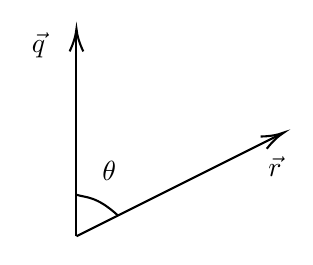
\begin{tikzpicture}[x=0.75pt,y=0.75pt,yscale=-1,xscale=1]
%uncomment if require: \path (0,300); %set diagram left start at 0, and has height of 300

%Straight Lines [id:da4402999370947803] 
\draw    (250,150) -- (250,52) ;
\draw [shift={(250,50)}, rotate = 90] [color={rgb, 255:red, 0; green, 0; blue, 0 }  ][line width=0.75]    (10.93,-3.29) .. controls (6.95,-1.4) and (3.31,-0.3) .. (0,0) .. controls (3.31,0.3) and (6.95,1.4) .. (10.93,3.29)   ;
%Straight Lines [id:da0037929251539179365] 
\draw    (250,150) -- (348.21,100.89) ;
\draw [shift={(350,100)}, rotate = 153.43] [color={rgb, 255:red, 0; green, 0; blue, 0 }  ][line width=0.75]    (10.93,-3.29) .. controls (6.95,-1.4) and (3.31,-0.3) .. (0,0) .. controls (3.31,0.3) and (6.95,1.4) .. (10.93,3.29)   ;
%Curve Lines [id:da06140636400336408] 
\draw    (250,130) .. controls (254.53,131.45) and (259.53,130.45) .. (270,140) ;

% Text Node
\draw (227,50.4) node [anchor=north west][inner sep=0.75pt]    {$\vec{q}$};
% Text Node
\draw (341,110.4) node [anchor=north west][inner sep=0.75pt]    {$\vec{r}$};
% Text Node
\draw (261,112.4) node [anchor=north west][inner sep=0.75pt]    {$\theta $};


\end{tikzpicture}
	\caption{Illustration of the angle between the two vectors $\vec{q}$ and $\vec{r}$ in equation (\ref{expansion})}
	\label{normsphere}
\end{marginfigure}
The final state consists of the unbound system represented by $\psi$. We know the final state consists of a plane wave with wave number $\vec{q}$ propagating along the $z$-axis. This can be represented by 
\begin{equation} \label{key}
	\text{e}^{iqz} = \text{e}^{i \vec{q}\cdot \vec{r}},
\end{equation}
where $\theta$ is the angle between $\vec{q}$ and $\vec{r}$ illustrated on \ref{normsphere}. Using orthogonality and the addition theorem for the spherical harmonics, we can decompose the plane wave into a Bessel function and spherical harmonics\footnote{This is proved in appendix \ref{app:Bessel}}. This yields
\begin{align}\label{planewaveexpansion}
	\frac{1}{\sqrt{V}} \text{e}^{-i\vec{q}\cdot\vec{r}} &= \frac{1}{\sqrt{V}} \sum_{\ell,m} 4\pi i^\ell Y_\ell^{*m}(\vec{q})Y_\ell^m(\vec{r})j_\ell(qr) \\
	&= \frac{1}{\sqrt{V}} \sum_\ell 4\pi i^\ell j_\ell(qr) \bigg( \frac{2\ell+1}{4\pi}\bigg)P_\ell(\cos\theta),
\end{align}
and $P_\ell$ is the Legendre polynomial of degree $\ell$. Since we are considering the energies close to the threshold, we expect mainly the $S$-wave to contribute and ignore higher orders. We should empathise that this is an approximation, and a priori, we do not know to what degree this holds. In terms of the expansion \eqref{planewaveexpansion} this greatly reduces the expression
\begin{equation} \label{expansion}
	\frac{1}{\sqrt{V}}\text{e}^{i\vec{q}\cdot \vec{r}} \stackrel{\ell=0}{=} \frac{1}{\sqrt{V}}j_0(qr).
\end{equation}
As equation \eqref{expansion} shows, we are left with a spherical Bessel function in the final state where the volume is kept to stress that according to (REF MISSING) the total cross section must be independent of the volume. Considering the $S$-wave channel for the following process $p \gamma \rightarrow n\pi^+$ yields the following matrix element
\begin{equation}
	\mathcal{M}=-i\omega_k\sqrt{\frac{2\pi\hbar}{V\omega_{\vec{k}}}}\vec{e}_{\vec{k},\lambda}\mel*{\frac{1}{\sqrt{V}} j_0(qr)n\pi^+ (\uparrow \downarrow)}{\vec{d}}{(\vec{\tau}\cdot \vec{\pi})(\vec{\sigma}\cdot \vec{r})p\uparrow \phi(r)\mathcal{N}}
\end{equation}
where the two arrows represent the two spin states of the neutron and the proton. The front factor arises from the normalisation factor in front of the 2nd quantisation operator. The different spin states of the neutron in the final state yield two contributions to the total matrix element given by
\begin{align}
	\mathcal{M}^{\uparrow} &=\frac{-i\mathcal{N}\sqrt{2}\omega_k\vec{e}_{\vec{k},\lambda}}{V}\sqrt{\frac{2\pi\hbar}{V\omega_{\vec{k}}}}\mel*{j_0(qr)}{d_0 r_0}{\phi(r)}  \\
	&= \frac{-i\mathcal{N}\sqrt{2}\omega_k\vec{e}_{\vec{k},\lambda}}{V}\sqrt{\frac{2\pi\hbar}{V\omega_{\vec{k}}}}\sqrt{\frac{4\pi}{3}}\mel*{j_0(qr)}{d_0 r Y_1^0}{\phi(r)} \\
	\mathcal{M}^{\downarrow} & = \frac{-i\mathcal{N}2\omega_k\vec{e}_{\vec{k},\lambda}}{V}\sqrt{\frac{2\pi\hbar}{V\omega_{\vec{k}}}} \mel{j_0(qr)}{d r_{+}}{\phi(r)}\\
	&=\frac{-i\mathcal{N}2\omega_k\vec{e}_{\vec{k},\lambda}}{V}\sqrt{\frac{2\pi\hbar}{V\omega_{\vec{k}}}}\sqrt{\frac{4\pi}{3}}\mel*{j_0(qr)}{d_0 r Y_1^1}{\phi(r)}, \\
\end{align}
where the spin-down state picks up a factor $\sqrt{2}$ from equation \eqref{spinmatrix}. Now we calculate the remaining matrix elements,
\begin{align}
	\mel{j_0(qr)}{d_0 r_0}{\phi(r)} &= \frac{\mu}{m_\pi}e \mel{j_0(qr)}{r_0r_0}{\phi(r)} \\
	&= \frac{\mu}{m_\pi}e\frac{4\pi}{3} \mel{j_0}{r^2}{\phi(r)} \\
	&= \frac{\mu e }{m_\pi} \int_0^\pi \int_0^{2\pi} \int_0^\infty \text{d}r \text{d}\phi \text{d}\theta \, j_0(qr)r^4\cos^2\theta \sin\theta \phi(r) \\
	&= \frac{4\pi \mu e}{3m_\pi} \underbrace{\int_0^\infty \text{d}r \, j_0(qr)r^4\phi(r)}_{\mathcal{Q}(r)}, \label{Matrix1}
\end{align}
where the dipole operator has been inserted and the angular integrals calculated. We have also introduced an integral, which contains the wave function $\phi(r)$. Similarly, for the next matrix element,
\begin{align}
	\mel{j_0(qr)}{d_{-}r_{+}}{\phi(r)} &= \frac{\mu}{m_\pi}e \mel{j_0(qr)}{r_{-}r_{+}}{\phi(r)} \\
	&= \frac{4\pi \mu e}{3 m_\pi} \mel{j_0(qr)}{r^2 Y_1^{-1}Y_1^1}{\phi(r)} \\
	&= \frac{4\pi \mu e}{3 m_\pi} \mathcal{Q}. \label{Matrix2}
\end{align}
It turns out these two matrix elements are equal. Taking the norm-square of \eqref{Matrix1}
\begin{equation}
	\abs{\mathcal{M}^\uparrow}^2 = \bigg( \frac{4\pi \mu e}{3m_\pi}\bigg)^2 \frac{2 \mathcal{N}^2\omega_k (2\pi \hbar)}{V^2}(\vec{e}_{\vec{k},\lambda})^0(\vec{e}_{\vec{k},\lambda}^*)^0 \mathcal{Q}^2 
\end{equation}
Similarly, for the equation \eqref{Matrix2}
\begin{equation}
	\abs{\mathcal{M}^\downarrow}^2 = \bigg( \frac{4\pi \mu e}{3 m_\pi}\bigg)^2 \frac{4\mathcal{N}\omega_{\vec{k}}(2\pi\hbar)}{V^2}(\vec{e}_{\vec{k},\lambda})^+(\vec{e}_{\vec{k},\lambda}^*)^+ \mathcal{Q}^2.
\end{equation}
Calculating the total matrix element using a polarization theorem\footnote{$(\vec{e}_{\vec{k},\lambda}^*\cdot \vec{e}_{\vec{k},\lambda})=\delta_{\lambda,\lambda'}$ and $\vec{e}_{\vec{k},\mp}=\pm\frac{1}{\sqrt{2}}(\vec{e}_{\vec{k},1}\pm i\vec{e}_{\vec{k},2})$. This leads to $(\vec{e}^{0*}_{\vec{k},\lambda}\cdot\vec{e}^{0}_{\vec{k},\lambda'})+(\vec{e}^{0+}_{\vec{k},\lambda}\cdot\vec{e}^{+}_{\vec{k},\lambda'})=\delta_{\lambda,\lambda'}+\frac{1}{2}\delta_{\lambda,\lambda'}$}
\begin{align}
	\abs{\mathcal{M}}^2 &= \abs{\mathcal{M}^\uparrow}^2 + \abs{\mathcal{M}^\downarrow}^2 \\
	&= \frac{2\pi \hbar \omega_k \mathcal{N}^2 e^2}{V^2} \bigg( \frac{4\pi\mu}{3m_\pi}\bigg)^2 \mathcal{Q}^2,
\end{align}
\begin{marginfigure}
	\centering
	

\tikzset{every picture/.style={line width=0.75pt}} %set default line width to 0.75pt        

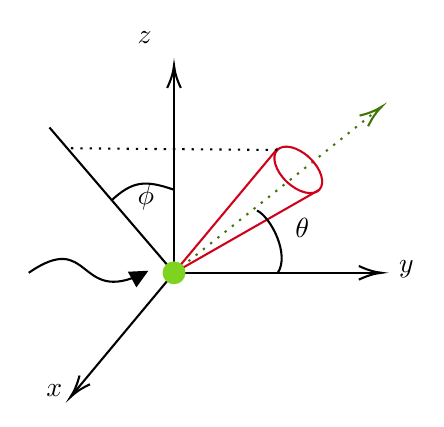
\begin{tikzpicture}[x=0.75pt,y=0.75pt,yscale=-1,xscale=1]
%uncomment if require: \path (0,362); %set diagram left start at 0, and has height of 362

%Straight Lines [id:da8075674552034334] 
\draw    (270,180) -- (210,110) ;
%Straight Lines [id:da1934453842044379] 
\draw [color={rgb, 255:red, 65; green, 117; blue, 5 }  ,draw opacity=1 ] [dash pattern={on 0.84pt off 2.51pt}]  (270,180) -- (368.44,101.25) ;
\draw [shift={(370,100)}, rotate = 141.34] [color={rgb, 255:red, 65; green, 117; blue, 5 }  ,draw opacity=1 ][line width=0.75]    (10.93,-3.29) .. controls (6.95,-1.4) and (3.31,-0.3) .. (0,0) .. controls (3.31,0.3) and (6.95,1.4) .. (10.93,3.29)   ;
%Straight Lines [id:da551977907100426] 
\draw [color={rgb, 255:red, 208; green, 2; blue, 27 }  ,draw opacity=1 ]   (270,180) -- (340,140) ;
%Straight Lines [id:da13834667273930523] 
\draw [color={rgb, 255:red, 208; green, 2; blue, 27 }  ,draw opacity=1 ]   (270,180) -- (320,120) ;
%Straight Lines [id:da575178064615293] 
\draw    (270,180) -- (270,82) ;
\draw [shift={(270,80)}, rotate = 90] [color={rgb, 255:red, 0; green, 0; blue, 0 }  ][line width=0.75]    (10.93,-3.29) .. controls (6.95,-1.4) and (3.31,-0.3) .. (0,0) .. controls (3.31,0.3) and (6.95,1.4) .. (10.93,3.29)   ;
%Straight Lines [id:da30763782233069703] 
\draw    (270,180) -- (368,180) ;
\draw [shift={(370,180)}, rotate = 180] [color={rgb, 255:red, 0; green, 0; blue, 0 }  ][line width=0.75]    (10.93,-3.29) .. controls (6.95,-1.4) and (3.31,-0.3) .. (0,0) .. controls (3.31,0.3) and (6.95,1.4) .. (10.93,3.29)   ;
%Straight Lines [id:da016368323591563816] 
\draw    (270,180) -- (221.28,238.46) ;
\draw [shift={(220,240)}, rotate = 309.81] [color={rgb, 255:red, 0; green, 0; blue, 0 }  ][line width=0.75]    (10.93,-3.29) .. controls (6.95,-1.4) and (3.31,-0.3) .. (0,0) .. controls (3.31,0.3) and (6.95,1.4) .. (10.93,3.29)   ;
%Curve Lines [id:da6672149281430028] 
\draw    (200,180) .. controls (230.55,158.88) and (223.07,196.06) .. (255.12,180.32) ;
\draw [shift={(257.67,179)}, rotate = 151.5] [fill={rgb, 255:red, 0; green, 0; blue, 0 }  ][line width=0.08]  [draw opacity=0] (8.93,-4.29) -- (0,0) -- (8.93,4.29) -- cycle    ;
%Flowchart: Connector [id:dp12078467552802752] 
\draw  [color={rgb, 255:red, 126; green, 211; blue, 33 }  ,draw opacity=1 ][fill={rgb, 255:red, 126; green, 211; blue, 33 }  ,fill opacity=1 ] (265,180) .. controls (265,177.24) and (267.24,175) .. (270,175) .. controls (272.76,175) and (275,177.24) .. (275,180) .. controls (275,182.76) and (272.76,185) .. (270,185) .. controls (267.24,185) and (265,182.76) .. (265,180) -- cycle ;
%Shape: Ellipse [id:dp45046333760686075] 
\draw  [color={rgb, 255:red, 208; green, 2; blue, 27 }  ,draw opacity=1 ] (319.75,120.83) .. controls (322.77,117.63) and (329.76,119.33) .. (335.35,124.63) .. controls (340.94,129.92) and (343.03,136.8) .. (340,140) .. controls (336.97,143.2) and (329.99,141.49) .. (324.4,136.2) .. controls (318.8,130.91) and (316.72,124.02) .. (319.75,120.83) -- cycle ;
%Straight Lines [id:da9664046710126799] 
\draw  [dash pattern={on 0.84pt off 2.51pt}]  (319.75,120.83) -- (220,120) ;
%Curve Lines [id:da6106413145156059] 
\draw    (310,150) .. controls (316.83,153.33) and (325.83,171.33) .. (320,180) ;
%Curve Lines [id:da19983569644229238] 
\draw    (240,145) .. controls (249.83,136) and (255.83,135) .. (270,140) ;

% Text Node
\draw (251,62.4) node [anchor=north west][inner sep=0.75pt]    {$z$};
% Text Node
\draw (377,172.4) node [anchor=north west][inner sep=0.75pt]    {$y$};
% Text Node
\draw (207,232.4) node [anchor=north west][inner sep=0.75pt]    {$x$};
% Text Node
\draw (327,152.4) node [anchor=north west][inner sep=0.75pt]    {$\theta $};
% Text Node
\draw (251,136.4) node [anchor=north west][inner sep=0.75pt]    {$\phi $};


\end{tikzpicture}
	\caption{Illustration of the differential cross-section. }
	\label{fig:diffcrossillustration}
\end{marginfigure}  
which is the final expression for the matrix element. According to Fermi's golden rule, we can calculate the transition probability
\begin{equation}\label{domega}
	\text{d}\omega = \frac{2\pi}{\hbar} \abs{\mathcal{M}}^2 \text{d}\rho,
\end{equation}
where the density of states is given by
\begin{equation}\label{densityofstates}
	\text{d}\rho = \frac{Vqm }{\hbar^2 (2\pi)^3}\text{d}\Omega.
\end{equation}
To go from the transition probability to the differential cross-section, we need to consider the flux density of the photons. This means a factor $V/c$, where $V$ is the volume, and $c$ is the speed of light. This leads to the final expressions for the differential cross-section.
\begin{equation}\label{diffcrosssection}
	\frac{\text{d}\sigma}{\text{d}\Omega_q}=\frac{16 \pi}{9} \mathcal{N}^2 \alpha\frac{kq\mu^3_{N\pi}}{m_\pi^2 \hbar c}\mathcal{Q}^2,
\end{equation}
and since there is no explicit angular dependency, the total cross-section is given by
\begin{align}
	\sigma_\text{dipole} & = \oint_{4\pi} \frac{\text{d}\sigma}{\text{d}\Omega_q} \text{d}\Omega_q \\
	&= 4\pi \frac{16 \pi}{9} \mathcal{N}^2 \alpha\frac{kq\mu^3_{N\pi}}{m_\pi^2 \hbar c}\mathcal{Q}^2 \\
	&= \frac{64\pi^2}{9}\mathcal{N}^2 \alpha \frac{kq\mu^3_{p\pi}}{m_\pi^2 \hbar c} \left( \int_0^\infty \text{d}r \, j_0(qr)r^4 \phi(r)\right)^2 \label{dipoletotalcross}.
\end{align}
This is the final expression for the total cross-section of photoproduction of charged pions using the dipole approximation. We now perform a fit to experimental data for the parameters $S$ and $b$ and enter in the wave function $\phi(r)$. Here two considerations are needed. Both the dipole approximation and the one-pion approximation limit the validity of the cross-section to near the threshold. And due to the limited amount of experimental data for charged pion photoproduction the fit is limited to approximately $15$ MeV from the threshold. This means some data points are excluded to constrain the fitted parameters to values that might seem physically realistic. 

The fit is performed and can be seen in figure \ref{fig:dipolefit}.
\begin{figure}[H]
	\begin{sidecaption}{The total cross-section of the photoproduction process $\gamma p \rightarrow \pi^+ n$ fitted to experimental data. The fit parameters are shown in the figure. The blue data points are included in the fit, and the black data points are excluded since these violate both the dipole and the one pion approximation.}[fig:dipolefit]
		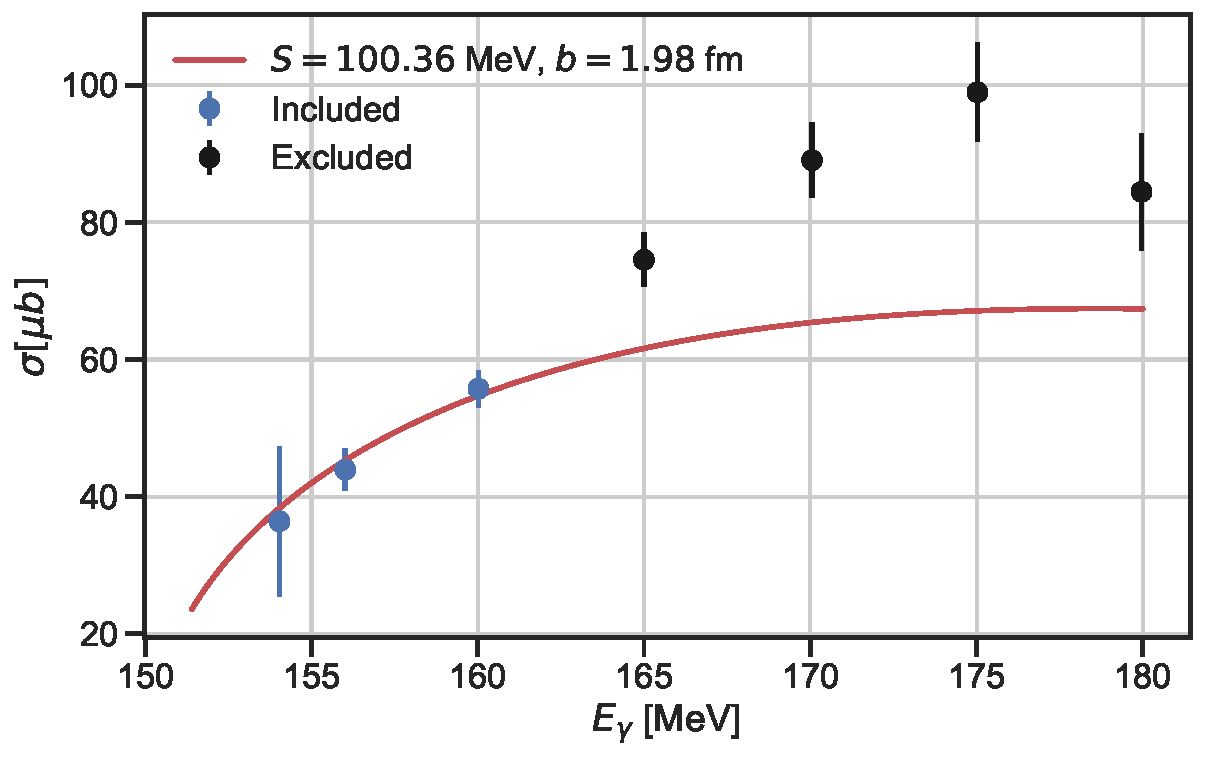
\includegraphics[width=\linewidth]{Figures/dipole_approximation.pdf}
	\end{sidecaption}
\end{figure}
The parameters $S$ and $b$ seem reasonable, but more importantly, we are interested in the relative weight coming from the $N\pi$ component in the wave function and the virtual pions' contribution to the dressed proton. This corresponds to solving the equations in \eqref{system} with the new parameters. The contribution to the wave function is calculated as follows
\begin{align}
	\int_V \text{d}^3R \int_V \text{d}^3 r \, \abs{\psi_{N\pi}}^2 &= 4\pi \int_0^\infty \text{d}r \, \phi(r)^2r^2 \\
	&= 0.69
\end{align}
using \eqref{pionnuc} and considering only the $\pi^+$ component in $\vec{\pi}$. The energy is calculated which yields
\begin{equation}
	E_{\text{virtual pions}} = -449 \, \text{MeV}.
\end{equation}
Note here that we have used two approximations that limit \eqref{dipoletotalcross} to energies very close to the threshold. To further test the validity of the model, we need a more general expression for the cross-section and more data points. This means we have to consider the exact matrix element for the transition and consider the photoproduction of neutral pions off protons since this is the most experimentally investigated photoproduction process. 
\section{Exact Matrix Element}\label{sec:exact}
In section \ref{sec:dipoleapprox} we looked at how to use the model described in section \ref{sec:model} to get an expression for the cross-section which was compared to experimental data. More specifically we used the dipole approximation which introduces a trade-off between the difficulty of the calculations and the regime in which our solution is valid. We expect the dipole approximation to hold for low energies just above the threshold. To both validate and generalize this result we now do a different approach and calculate the cross-section exact and also consider recoil effects. Strictly speaking, recoil effects should also be considered in section \ref{sec:dipoleapprox} since the mass ratio between the nucleon and the pion cannot be assumed to yield a stationary nucleon after the pion photoproduction process. To calculate the exact matrix elements we consider a non-relativistic system of particles interacting with the electromagnetic field. The interacting part of the Hamiltonian is given by
\begin{equation} \label{firstinthamil}
	H = \frac{1}{2m_\pi} \bigg( \vec{p}-\frac{e}{c}\vec{A}(\vec{r}) \bigg)^2,
\end{equation}
where $\vec{p}$ is the momentum operator and $\vec{A}(\vec{r})$ is the quantized vector potential at the point $\vec{r}$. Note that we have already replaced the usual mass by the mass of the pion, $m_\pi$ since we are considering the interaction of a pion with charge $e$ with the electromagnetic field. 

The electromagnetic interaction is relatively weak compared to the strong force. For our problem, this means we can expand the interaction by taking only the lowest non-vanishing order of perturbation into account. Since we later want to consider transition probabilities we only keep the first non-linear term of \eqref{firstinthamil} which yields
\begin{equation}\label{secondinthamil}
	V^{(1)} = -\frac{e}{2m_p c}\bigg( \vec{p}\cdot \vec{A}(\vec{r}_p,t)+\vec{A}(\vec{r}_p,t)\cdot \vec{p}\bigg),
\end{equation}
\begin{marginfigure}
	\centering
	

\tikzset{every picture/.style={line width=0.75pt}} %set default line width to 0.75pt        

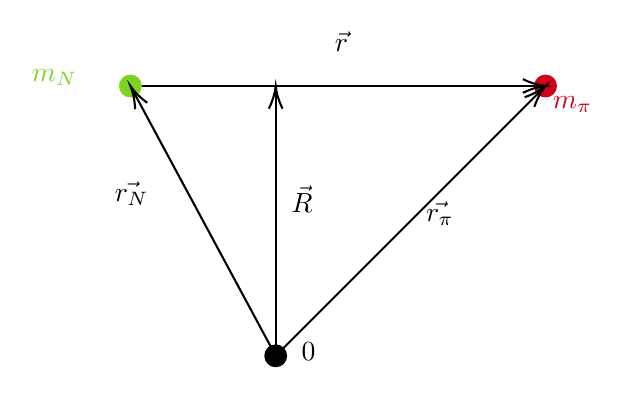
\begin{tikzpicture}[x=0.75pt,y=0.75pt,yscale=-1,xscale=1]
	%uncomment if require: \path (0,300); %set diagram left start at 0, and has height of 300
	
	%Flowchart: Connector [id:dp9827455772611288] 
	\draw  [color={rgb, 255:red, 208; green, 2; blue, 27 }  ,draw opacity=1 ][fill={rgb, 255:red, 208; green, 2; blue, 27 }  ,fill opacity=1 ] (315,90) .. controls (315,87.24) and (317.24,85) .. (320,85) .. controls (322.76,85) and (325,87.24) .. (325,90) .. controls (325,92.76) and (322.76,95) .. (320,95) .. controls (317.24,95) and (315,92.76) .. (315,90) -- cycle ;
	%Straight Lines [id:da5093684133345362] 
	\draw    (125,90) -- (318,90) ;
	\draw [shift={(320,90)}, rotate = 180] [color={rgb, 255:red, 0; green, 0; blue, 0 }  ][line width=0.75]    (10.93,-3.29) .. controls (6.95,-1.4) and (3.31,-0.3) .. (0,0) .. controls (3.31,0.3) and (6.95,1.4) .. (10.93,3.29)   ;
	%Straight Lines [id:da04984112064582158] 
	\draw    (190,220) -- (190,92) ;
	\draw [shift={(190,90)}, rotate = 90] [color={rgb, 255:red, 0; green, 0; blue, 0 }  ][line width=0.75]    (10.93,-3.29) .. controls (6.95,-1.4) and (3.31,-0.3) .. (0,0) .. controls (3.31,0.3) and (6.95,1.4) .. (10.93,3.29)   ;
	%Straight Lines [id:da13661676787341415] 
	\draw    (190,220) -- (318.59,91.41) ;
	\draw [shift={(320,90)}, rotate = 135] [color={rgb, 255:red, 0; green, 0; blue, 0 }  ][line width=0.75]    (10.93,-3.29) .. controls (6.95,-1.4) and (3.31,-0.3) .. (0,0) .. controls (3.31,0.3) and (6.95,1.4) .. (10.93,3.29)   ;
	%Flowchart: Connector [id:dp37210275318157304] 
	\draw  [color={rgb, 255:red, 126; green, 211; blue, 33 }  ,draw opacity=1 ][fill={rgb, 255:red, 126; green, 211; blue, 33 }  ,fill opacity=1 ] (115,90) .. controls (115,87.24) and (117.24,85) .. (120,85) .. controls (122.76,85) and (125,87.24) .. (125,90) .. controls (125,92.76) and (122.76,95) .. (120,95) .. controls (117.24,95) and (115,92.76) .. (115,90) -- cycle ;
	%Straight Lines [id:da8769015497622031] 
	\draw    (190,220) -- (120.95,91.76) ;
	\draw [shift={(120,90)}, rotate = 61.7] [color={rgb, 255:red, 0; green, 0; blue, 0 }  ][line width=0.75]    (10.93,-3.29) .. controls (6.95,-1.4) and (3.31,-0.3) .. (0,0) .. controls (3.31,0.3) and (6.95,1.4) .. (10.93,3.29)   ;
	%Flowchart: Connector [id:dp5562170943538245] 
	\draw  [color={rgb, 255:red, 0; green, 0; blue, 0 }  ,draw opacity=1 ][fill={rgb, 255:red, 0; green, 0; blue, 0 }  ,fill opacity=1 ] (185,220) .. controls (185,217.24) and (187.24,215) .. (190,215) .. controls (192.76,215) and (195,217.24) .. (195,220) .. controls (195,222.76) and (192.76,225) .. (190,225) .. controls (187.24,225) and (185,222.76) .. (185,220) -- cycle ;
	
	% Text Node
	\draw (71,80.4) node [anchor=north west][inner sep=0.75pt]  [color={rgb, 255:red, 126; green, 211; blue, 33 }  ,opacity=1 ]  {$m_{N}$};
	% Text Node
	\draw (322,93.4) node [anchor=north west][inner sep=0.75pt]  [color={rgb, 255:red, 208; green, 2; blue, 27 }  ,opacity=1 ]  {$m_{\pi }$};
	% Text Node
	\draw (196,136.4) node [anchor=north west][inner sep=0.75pt]    {$\vec{R}$};
	% Text Node
	\draw (261,144.4) node [anchor=north west][inner sep=0.75pt]    {$\vec{r_{\pi }}$};
	% Text Node
	\draw (111,134.4) node [anchor=north west][inner sep=0.75pt]    {$\vec{r_{N}}$};
	% Text Node
	\draw (217,62.4) node [anchor=north west][inner sep=0.75pt]    {$\vec{r}$};
	% Text Node
	\draw (201,212.4) node [anchor=north west][inner sep=0.75pt]    {$0$};
	
	
\end{tikzpicture}
	\caption{Jacobi coordinates illustrating $\vec{r}_\pi$ used in the vector potential in equation \ref{thirdinthamil}. Here we use $\vec{r}=\vec{r}_\pi-\vec{r}_p$ and see that $\vec{r}_\pi = \vec{R}+\vec{r}\frac{m_p}{M_{p \pi}}$, where $M_{p\pi}=m_p+m_\pi$.}
	\label{JacobiIllustration}
\end{marginfigure}
\noindent which also means the interacting part is linear in the creation(annihilation) operators corresponding to single-photon emission(absorption). Our choice of gauge is purely conventional and we choose the radiation gauge which imposes a condition on the vector potential given by
\begin{equation}
	\nabla \cdot \vec{A} = 0,
\end{equation}
and this is a convenient choice of gauge since the commutator in \eqref{secondinthamil} is $\nabla \cdot \vec{A}$ and we can write
\begin{equation}\label{thirdinthamil}
	V^{(1)} = -\frac{e}{m_p c}\vec{A}(\vec{r_p},t)\cdot \vec{p}_p. 
\end{equation}
Note that \eqref{thirdinthamil} consists of the pion momentum operator, $\vec{p}_\pi$ and the electromagnetic vector potential at a distance $r_\pi$. This distance was also mentioned in section \ref{sec:model} and can be expressed in term of the Jacobi coordinates illustrated on figure \ref{JacobiIllustration} where the relative coordinate is given by $\vec{r}=\vec{r}_\pi-\vec{r}_p$ which leads to the following transformation of equation \eqref{thirdinthamil}
\begin{equation}
	V^{(1)} = -\frac{e}{m_p c}\vec{A}(\vec{r_p},t)\cdot \vec{p}_p = -\frac{e}{m_p c} \vec{A}\bigg( \vec{R}-\frac{m_\pi}{M_{p\pi}}\vec{r},t\bigg)\bigg(\frac{m_p}{M_{p\pi}}\vec{P}-\vec{p}\bigg),
\end{equation}
where $M_{p \pi}=m_p+m_\pi$ is the total mass of the system and $\vec{R}$ is the coordinate vector for the center of mass. We now move on from the general theory of the pion interacting with the electromagnetic field and consider the specific case of pion photoproduction. To recap we consider the following processes
\begin{align}
	p \gamma & \rightarrow p \pi^0 \label{photo1}\\
	p \gamma & \rightarrow n \pi^+ \label{photo2}\\
	n \gamma & \rightarrow n \pi^0 \label{photo3}\\
	n \gamma & \rightarrow p \pi^- \label{photo4},
\end{align}
where the initial states consist of a dressed proton or neutron and a plane wave photon which in the language of 2nd quantization can be written as $a_{\vec{k},\lambda}^\dagger \ket{0}$ corresponding to creating a photon with wave vector $\vec{k}$ and polarization $\lambda$ from the vacuum $\ket{0}$. The final states consists of a nucleon and a pion and no photon, i.e electromagnetic vacuum. This leads to the following expression for the matrix element for the transitions in \eqref{photo1}, \eqref{photo2}, \eqref{photo3} and \eqref{photo4}
\begin{equation}\label{transitions}
	\frac{-e}{m_\pi c}\mel*{0}{\vec{A}\big( \vec{R}-\frac{m_\pi}{M_{p\pi}}\vec{r},t\big) a_{\vec{k},\lambda}^\dagger}{0} = \frac{-e}{m_p} \sqrt{\frac{2\pi \hbar}{\omega_{\vec{k}}V}} \vec{e}_{\vec{k},\lambda}\text{e}^{i\vec{k}(\vec{R}-\frac{m_\pi}{M_{p\pi}}\vec{r})-i\omega_k t}.
\end{equation}
Completely analogous to section \ref{sec:dipoles} and specifically equation \eqref{domega} we now want to consider the probability of transition per unit time of going from the initial state $\ket{i}$ to $\bra{f}$ according to Fermi's golden rule
\begin{equation}
	\text{d}\omega = \frac{2\pi}{\hbar} \abs{\mathcal{M}}^2 \text{d}\rho,
\end{equation}
where $\text{d}\rho$ is the density of states also analogous to \eqref{densityofstates}. The difference is that we do not employ the dipole approximation to evaluate the matrix element $\mathcal{M}$ and we also consider recoil. In the following section we focus on pion photoproduction of neutral pion off protons corresponding to the transition in \eqref{photo1}. The choice is due to the fact that there is a lot more experimental data available for pion photoproduction off protons compared to neutrons since it is easier to achive experimentally. We focus on neutral pions since our one-pion approximation is assumed to be valid near the threshold and since we are interested in fitting to experimental data we need as much data near the threshold as possible--and this is the case for neutral pion photoproduction
\subsection{Neutral Pion Phototoproduction off Protons}
From \eqref{transitions} we get
\begin{align}\label{MatrixSpinupdown} 
	\mathcal{M}^{(\uparrow\downarrow)} & = \frac{e}{m_p} \sqrt{\frac{2\pi\hbar}{\omega_{\vec{k}}V}} \mel*{(\uparrow\downarrow)p\pi^0 \frac{\text{e}^{i\vec{q}\cdot \vec{r}}}{\sqrt{V}}\frac{\text{e}^{i\vec{Q}\cdot \vec{r}}}{\sqrt{V}}}{\text{e}^{i\vec{k}(R-\frac{m_\pi}{M_{p\pi}}\vec{r})}(\vec{e}_{\vec{k},\lambda}\vec{p})}{(\vec{\tau}\cdot\vec{\pi})(\vec{\sigma}\cdot\vec{r})\phi(r) \frac{p\uparrow}{\sqrt{V}}} \\
	&= \frac{-e}{m_p} \sqrt{\frac{2\pi\hbar}{\omega_{\vec{k}}V}} \mel*{(\uparrow\downarrow) \frac{\text{e}^{i\vec{q}\cdot \vec{r}}}{\sqrt{V}}\frac{\text{e}^{i\vec{Q}\cdot \vec{r}}}{\sqrt{V}}}{\text{e}^{i\vec{k}(R-\frac{m_\pi}{M_{p\pi}}\vec{r})}(\vec{e}_{\vec{k},\lambda}\vec{p})}{(\vec{\sigma}\cdot\vec{r})\phi(r) \frac{\uparrow}{\sqrt{V}}} \label{MatrixSpinupdown2},
\end{align} 
\begin{marginfigure}
	\centering
	

\tikzset{every picture/.style={line width=0.75pt}} %set default line width to 0.75pt        

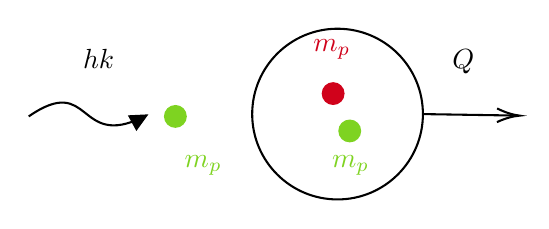
\begin{tikzpicture}[x=0.75pt,y=0.75pt,yscale=-1,xscale=1]
%uncomment if require: \path (0,408); %set diagram left start at 0, and has height of 408

%Curve Lines [id:da5989822671081096] 
\draw    (50.33,146) .. controls (80.88,124.88) and (73.41,162.06) .. (105.46,146.32) ;
\draw [shift={(108,145)}, rotate = 151.5] [fill={rgb, 255:red, 0; green, 0; blue, 0 }  ][line width=0.08]  [draw opacity=0] (8.93,-4.29) -- (0,0) -- (8.93,4.29) -- cycle    ;
%Flowchart: Connector [id:dp08119567255108817] 
\draw  [color={rgb, 255:red, 126; green, 211; blue, 33 }  ,draw opacity=1 ][fill={rgb, 255:red, 126; green, 211; blue, 33 }  ,fill opacity=1 ] (116,146) .. controls (116,143.24) and (118.24,141) .. (121,141) .. controls (123.76,141) and (126,143.24) .. (126,146) .. controls (126,148.76) and (123.76,151) .. (121,151) .. controls (118.24,151) and (116,148.76) .. (116,146) -- cycle ;
%Flowchart: Connector [id:dp04975844425187159] 
\draw  [color={rgb, 255:red, 208; green, 2; blue, 27 }  ,draw opacity=1 ][fill={rgb, 255:red, 208; green, 2; blue, 27 }  ,fill opacity=1 ] (192,135) .. controls (192,132.24) and (194.24,130) .. (197,130) .. controls (199.76,130) and (202,132.24) .. (202,135) .. controls (202,137.76) and (199.76,140) .. (197,140) .. controls (194.24,140) and (192,137.76) .. (192,135) -- cycle ;
%Flowchart: Connector [id:dp029263123361565446] 
\draw  [color={rgb, 255:red, 126; green, 211; blue, 33 }  ,draw opacity=1 ][fill={rgb, 255:red, 126; green, 211; blue, 33 }  ,fill opacity=1 ] (200,153) .. controls (200,150.24) and (202.24,148) .. (205,148) .. controls (207.76,148) and (210,150.24) .. (210,153) .. controls (210,155.76) and (207.76,158) .. (205,158) .. controls (202.24,158) and (200,155.76) .. (200,153) -- cycle ;
%Shape: Circle [id:dp6718718103888768] 
\draw   (158,144.88) .. controls (158,122.16) and (176.41,103.75) .. (199.12,103.75) .. controls (221.84,103.75) and (240.25,122.16) .. (240.25,144.88) .. controls (240.25,167.59) and (221.84,186) .. (199.12,186) .. controls (176.41,186) and (158,167.59) .. (158,144.88) -- cycle ;
%Straight Lines [id:da24501455375525605] 
\draw    (240.25,144.88) -- (284.89,145.59) ;
\draw [shift={(286.89,145.63)}, rotate = 180.92] [color={rgb, 255:red, 0; green, 0; blue, 0 }  ][line width=0.75]    (10.93,-3.29) .. controls (6.95,-1.4) and (3.31,-0.3) .. (0,0) .. controls (3.31,0.3) and (6.95,1.4) .. (10.93,3.29)   ;

% Text Node
\draw (75,112.4) node [anchor=north west][inner sep=0.75pt]    {$hk$};
% Text Node
\draw (124,163.4) node [anchor=north west][inner sep=0.75pt]  [color={rgb, 255:red, 126; green, 211; blue, 33 }  ,opacity=1 ]  {$m_{p}$};
% Text Node
\draw (195,163.4) node [anchor=north west][inner sep=0.75pt]  [color={rgb, 255:red, 126; green, 211; blue, 33 }  ,opacity=1 ]  {$m_{p}$};
% Text Node
\draw (186,107.4) node [anchor=north west][inner sep=0.75pt]  [color={rgb, 255:red, 208; green, 2; blue, 27 }  ,opacity=1 ]  {$m_{p}$};
% Text Node
\draw (253,112.4) node [anchor=north west][inner sep=0.75pt]    {$Q$};


\end{tikzpicture}
	\caption{Neutral pion photoproduction with conservation of momentum $\vec{k}=\vec{Q}$ illustrated}
	\label{qkenergy}
\end{marginfigure}
where we have used $\int \text{d}^3 r \text{e}^{i\vec{k}\cdot\vec{R}}=V$ and $\mel{p\pi^0}{\vec{\tau}\cdot\vec{\pi}}{p}=1$. Note that $\vec{q}$ is the wave-number of the pion-proton relative momentum and $\vec{Q}$ is originates from conservation of momentum, that is $\vec{Q}=\vec{k}$. Defining a new vector, $\vec{s}=\vec{q}+\frac{m_\pi}{M_{p\pi}}\vec{k}$ yields
\begin{equation}
    \mathcal{M}^{(\uparrow\downarrow)} = \frac{-e}{m_\pi} \sqrt{\frac{2\pi\hbar}{\omega_{\vec{k}}}} \frac{1}{V} \mel*{(\uparrow \downarrow)}{\mel*{\text{e}^{i\vec{s}\cdot\vec{r}}}{(\vec{e}_{\vec{k},\lambda}\vec{p})(\vec{\sigma}\cdot\vec{r})}{\phi(r)}}{\uparrow}
\end{equation}
Note the different inner products. We now do the plane wave expansion using \eqref{planewaveexpansion} and consider the angular averaging of two coordinates variables\footnote{$\int \text{d}\Omega \, n_k n_l =\frac{4\pi}{3}\delta_{kl}$, which means $\int \text{d}\Omega \, r_k r_l =\frac{4\pi r^2}{3}\delta_{kl}$, where $n$ is a unit vector}
\begin{align}
    \mel*{\text{e}^{i\vec{s}\cdot\vec{r}}}{(\vec{e}_{\vec{k},\lambda}\frac{\partial}{\partial \vec{r}})\sigmar}{\phi(r)} &=+i(\vec{e}_{\vec{k},\lambda}\cdot \vec{s}) \int \text{d}^3 r \, \text{e}^{i\vec{s}\cdot\vec{r}}\sigmar \phi(r) \\ 
    &= -i(\vec{e}_{\vec{k},\lambda}\cdot \vec{s}) \int \text{d}^3 r \, 3 i r j_1(sr) \frac{\vec{s}\cdot \vec{r}}{sr}\sigmar \phi(r) \\
    &= (\vec{e}_{\vec{k},\lambda}\cdot \vec{s})\sigmar \underbrace{\frac{4\pi}{s} \int_0^\infty \text{d}r \, r^3 j_1(sr) \phi(r)}_{F(s)}  \\
    &= (\vec{e}_{\vec{k},\lambda}\cdot \vec{s})\sigmar F(s).
\end{align}
Returning to the matrix element \eqref{MatrixSpinupdown2}
\begin{align}
    \mathcal{M^{(\uparrow\downarrow)}} &= \frac{ie\hbar}{m_p}\sqrt{\frac{2\pi \hbar}{\omega_k}}\frac{1}{V}\mel*{(\uparrow\downarrow)}{(\vec{e}_{\vec{k},\lambda}\cdot\vec{s})F(s)}{\uparrow} \\
    &=\frac{ie\hbar}{m_p}\sqrt{\frac{2\pi \hbar}{\omega_k}}\frac{1}{V} (\vec{e}_{\vec{k},\lambda}\cdot\vec{s})\mel*{(\uparrow\downarrow)}{\sigmar}{\uparrow}F(s),
\end{align}
which leads to the following expression for the norm square\footnote{We do this step already to use a completeness relation for the polarization.}
\begin{equation} \label{matrixspinupdownabs}
    \abs{\mathcal{M}^{(\uparrow\downarrow)}}^2 = \frac{2\pi\hbar^3e^2}{m_p^2\omega_k V^2} \abs{\evec\cdot \vec{s}}^2 \abs{\mel*{(\uparrow\downarrow)}{\sigmar}{\uparrow}}^2 F(s)^2,
\end{equation}
and now calculating
\begin{align} \label{sumoverpol}
    \sum_\lambda &= \abs{(\evec \cdot \vec{s})}^2 = \sum_\lambda (\evec^*\cdot \vec{s})(\evec\cdot\vec{s}) \\
    &= s^2 -\frac{(\vec{k}\cdot \vec{s})^2}{k^2} \\
    &= q^2 -\frac{(\vec{k}\cdot \vec{q})^2}{k^2} \\
    &= q^2 \sin^2(\theta_q),
\end{align}
where $\theta_q$ is the angle between $\vec{k}$ and $\vec{q}$ and we now have an angular dependency originating from the dot product. I have added a subscript $q$ to empathize that this relative to the final state momentum $\vec{q}$ located in $(\theta, \phi)$ also illustrated on figure \ref{fig:diffcrossillustration}.

Plugging \eqref{sumoverpol} into \eqref{matrixspinupdownabs} yields
\begin{equation} \label{absmatrixexact}
    \frac{1}{2}\sum_{\lambda,(\uparrow\downarrow)} \abs{\mathcal{M}_{fi}}^2 = \frac{\pi e^2\hbar^3}{V^2 m_p^2}\frac{1}{\omega_k} q^2\sin^2(\theta) s^2 F(s)^2.
\end{equation}
According to Fermi's golden rule the transition probability is given by
\begin{align}\label{Fermisgolden}
    \text{d}\omega &= \frac{2\pi}{\hbar}\abs{\mathcal{M}}^2\text{d}\rho, \quad \text{d}\rho = \frac{V \mu_{p\pi }q}{\hbar^2(2\pi)^3}\text{d}\Omega_q,
\end{align}
where the density of states in the final state assumes a non-relativistic expansion. Strictly speaking this is an approximation. Also, $\vec{q}$ denotes the differential angle element to empathize that this is relative to the pion-proton system. Plugging \eqref{absmatrixexact} into \eqref{Fermisgolden}
\begin{align}
    \text{d}\omega = \frac{e^2}{8\pi}\frac{\mu_{p\pi }c^2}{m_p^2 c^4 \omega_k}q^3 \sin^2(\theta_q) s^2 F(s)^2 \text{d}\Omega_q
\end{align}
which leads to the following expression for the differential cross section by considering the time it takes the photon to cross the volume, $V$.
\begin{align}\label{exactdiffcross}
    \frac{\text{d}\sigma}{\text{d}\Omega_q} &= \frac{e^2}{8\pi}\frac{\mu_{p\pi}c^2}{m_p^2c^4}\frac{q^3}{k}\sin^2(\theta_q) s^2 F(s)^2
\end{align}
In \eqref{exactdiffcross} we have an expression for the angular dependency. This means for some photon energy we get an angular distribution. This can also be compared to experimental data. (This can be done for all the figures in \cite[]{Beck_1990} and also for charged pions). Figure \ref{fig:angular151} shows the differential cross section as a function of the angle $\theta_{\text{cm}}$ compared to experimental data.  
\begin{figure}[H]
    \begin{sidecaption}{Not fitted parameters! Note the dependency is not $\sin(\theta_q)^2$ since there is a contribution from $F(s)$ as well.}[fig:angular151]
    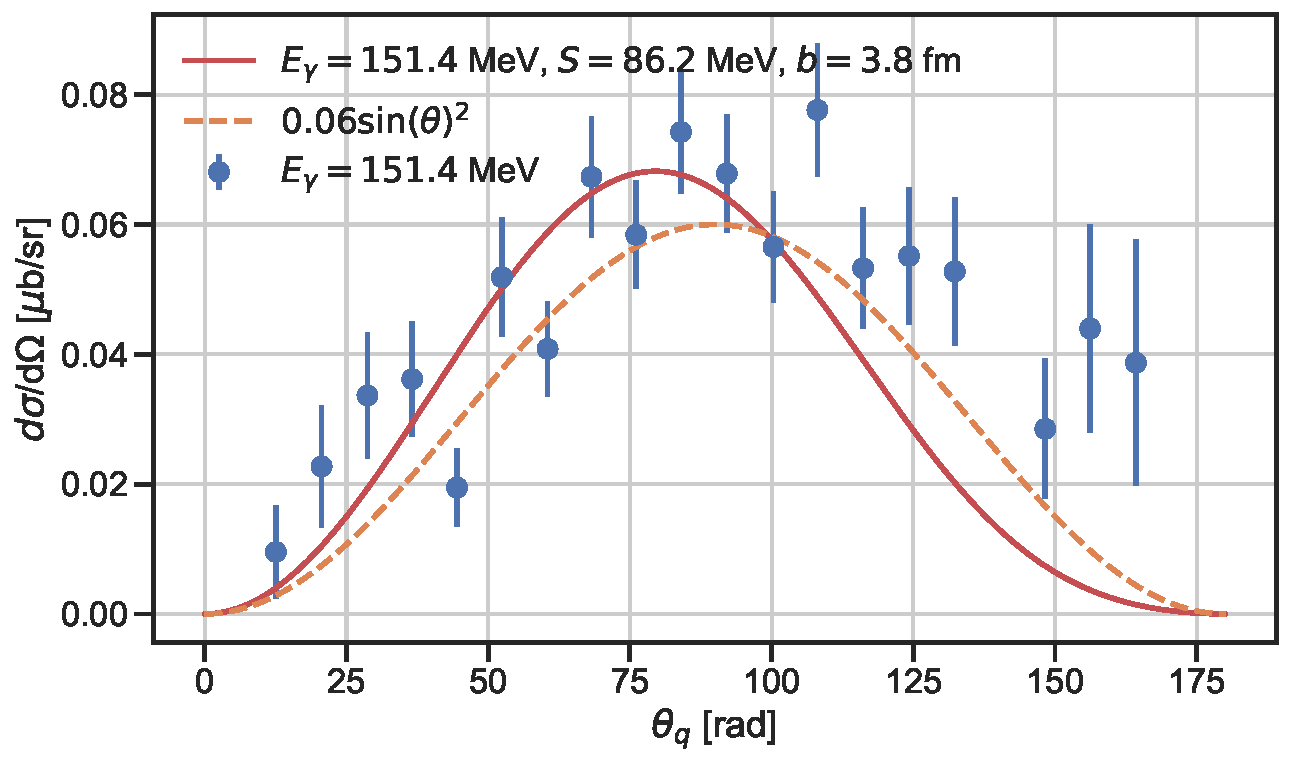
\includegraphics[width=\linewidth]{Figures/DiffCross151.pdf}
    \end{sidecaption}
\end{figure}
\begin{figure}[H]
    \begin{sidecaption}{Multiple energies}[fig:MultipleEnergies]
    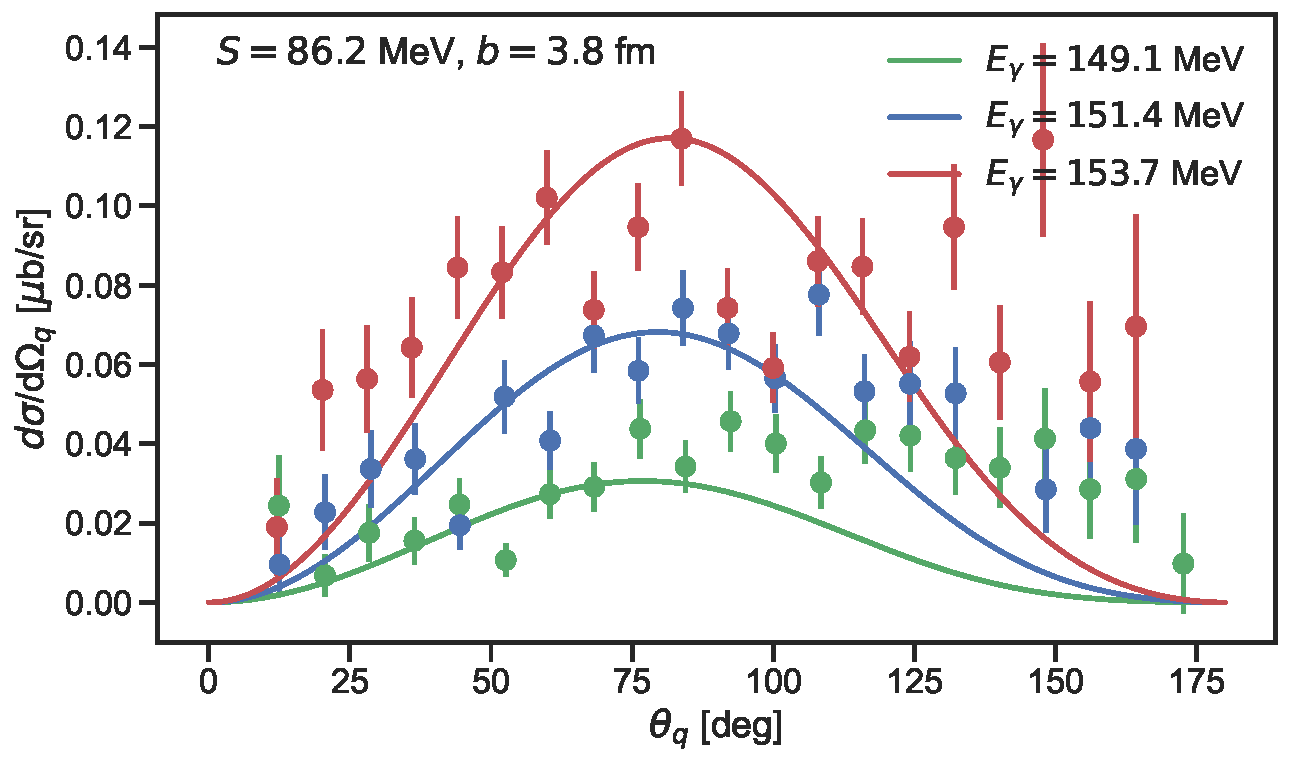
\includegraphics[width=\linewidth]{Figures/MultiDiffcross.pdf}
    \end{sidecaption}
\end{figure}
To get an expression for the total cross section equation the expression is integrated into containing only a radial part using
\begin{align} \label{exactcross}
    \sigma & = 2\pi \int_0^\pi \text{d}\theta \, \sin(\theta_q) \frac{\text{d}\sigma}{\text{d}\Omega_q} \\ &= 2\pi \int_0^\pi \text{d}\theta \, \frac{e^2}{8\pi}\frac{\mu_{p\pi}c^2}{m_p^2c^4}\frac{q^3}{k}\sin^3(\theta) s^2 F(s)^2
\end{align}
\eqref{exactcross} is fitted to experimental data such that the physical parameters in our model $S$ and $b$ can be extracted. So far the values of these parameters have been chosen at random. However, we do have some intuition about how these two affect the wavefunction of the system from figure \ref{fig:relativistic_expansion}. From \eqref{exactcross} we see that the wave function only enters explicitly in the integral so the general behavior of the cross section is hard to predict. The fit is done and can be seen in figure \ref{fig:crossfit}. Data is from \cite[]{Schmidt_2001}
\begin{figure}[H]
    \begin{sidecaption}{Fitted parameters to experimental data for the process $\gamma p \rightarrow \pi^0 p$. The fit parameters for $S,b$ are shown inside the figure.}[fig:crossfit]
    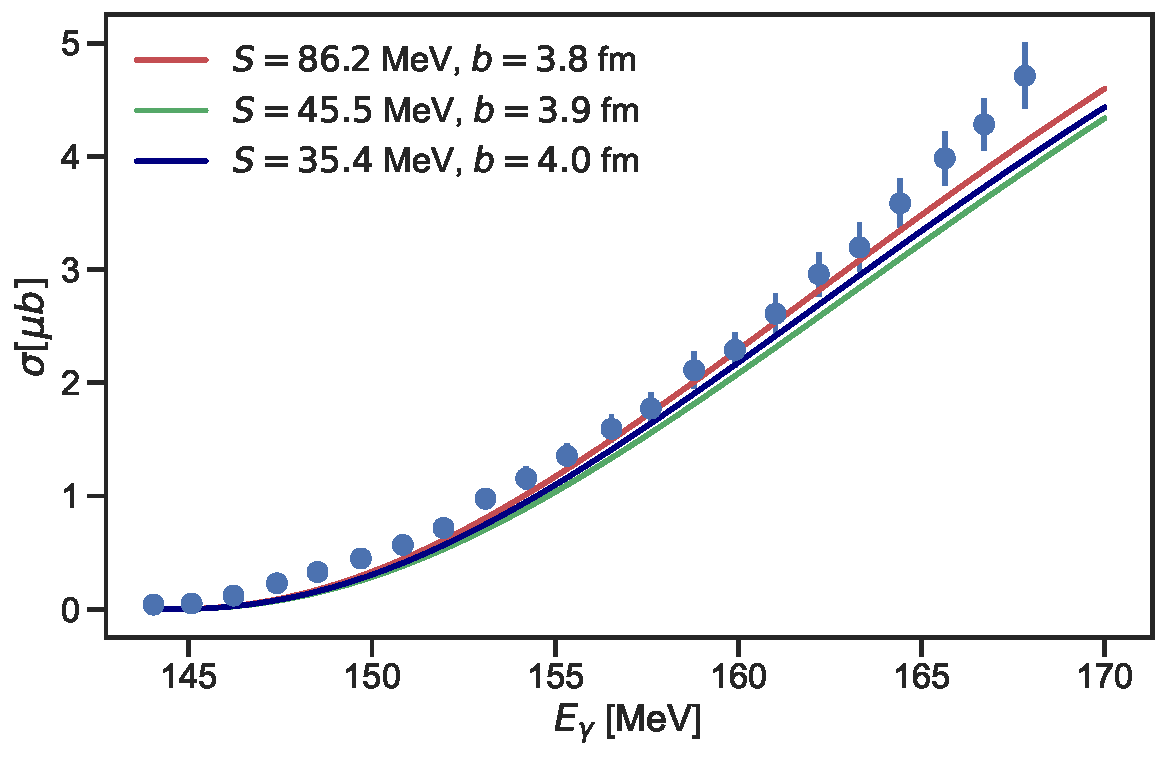
\includegraphics[width=\linewidth]{Figures/crossfit.pdf}
    \end{sidecaption}
\end{figure}
Note that these expressions are for the production of neutral pions. The same approach can be done for charged pions.

There is some freedom of choice in the fit. The integral is slowly converging and a cut-off must be introduced. This cut-off is arbitrary and does affect the fit. For a larger cut-off the line flattens out before 165 MeV. This leads to a more phenomenological discussion of the model in relation to the cross section as a function of energy. For higher energies we expect more than one pion to contribute to the cross section. This model, however, only takes one pion into account. To describe the behavior at higher energies more pions must be taking into account. This highlights the strengths and weaknesses of using differential equations to describe the physical system. If we take more pions into account this approach is no longer favorable since this leads to too many coupled systems. For more pions one would have to resort to another method.

\subsection{Neutral Pion Phototoproduction off Neutrons}
\begin{figure}[H]
    \begin{sidecaption}{The process $\gamma n \rightarrow \pi^0 n$ with the same parameters as for neutral pion photoproduction off protons.}[fig:neutralpionsoffneutrons]
    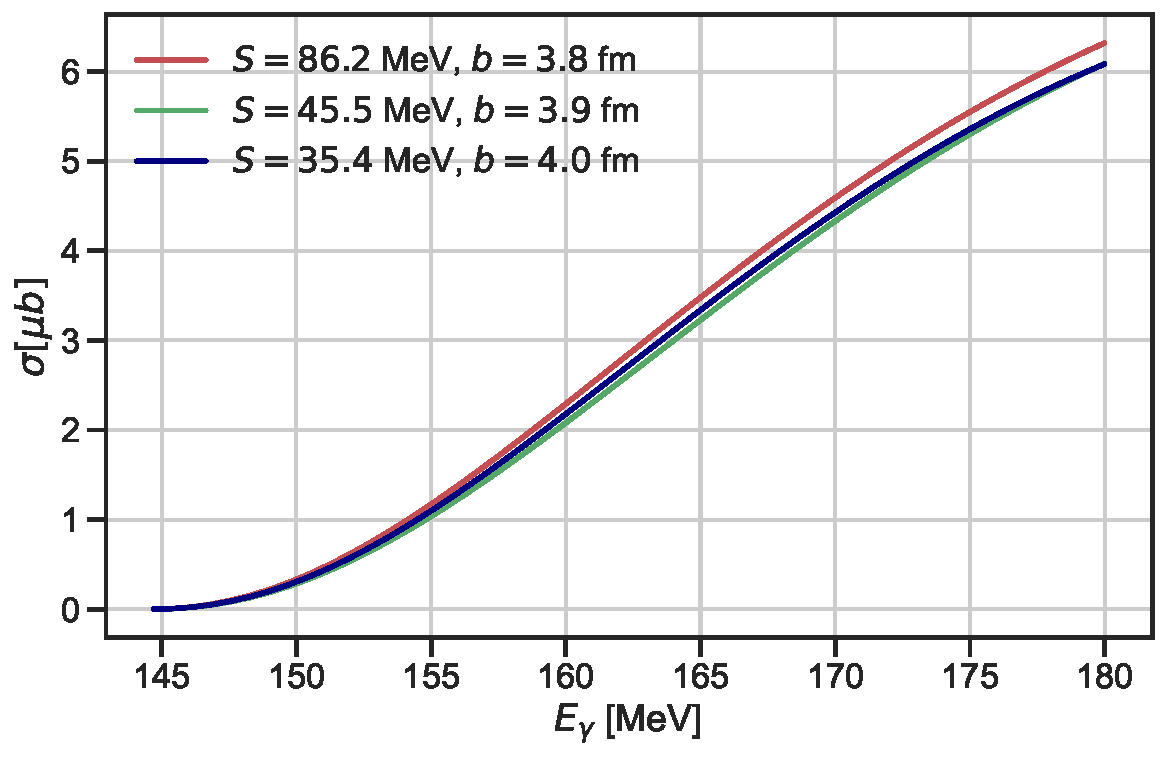
\includegraphics[width=\linewidth]{Figures/NeutralPionsOffNeutrons.pdf}
    \end{sidecaption}
\end{figure}
\subsection{Charged Pion Phototoproduction off Protons}
\subsection{Charged Pion Phototoproduction off Neutrons}